
% ------------------------------------------------------------
% ------------------------------------------------------------

%%%%%%%%%%%%%%%%%%%%%%%%%%%%%%%%%%%%%

% Section: Plots of TS in R 

\section[Time Series Plots]{Time Series Plots}
%%%%%%%%%%%%%%%%%%%%%%%%%%%%%%%%%%%%%

%\subsection{Univariate Plots}
%%%%%%%%%%%%%%%%%%%%%%%%%%%%%%%%%%%%%%

%\begin{frame}[fragile]
% \frametitle{Univariate Time Series Plot  \footnote{This section is from the SCC Mini-Course "Introductory Time Series \\ with R" by Irina Kukuyeva}}

%To plot one variables one at a time, use \ttfamily plot(): \normalfont 
%    \begin{columns}
%      \column{0.55\textwidth}
%		\begin{lstlisting}
%data(EuStockMarkets)
%dax<-EuStockMarkets[, 1]
%plot(dax)
%		\end{lstlisting}

%      \column{0.45\textwidth}
%       \begin{center}
%         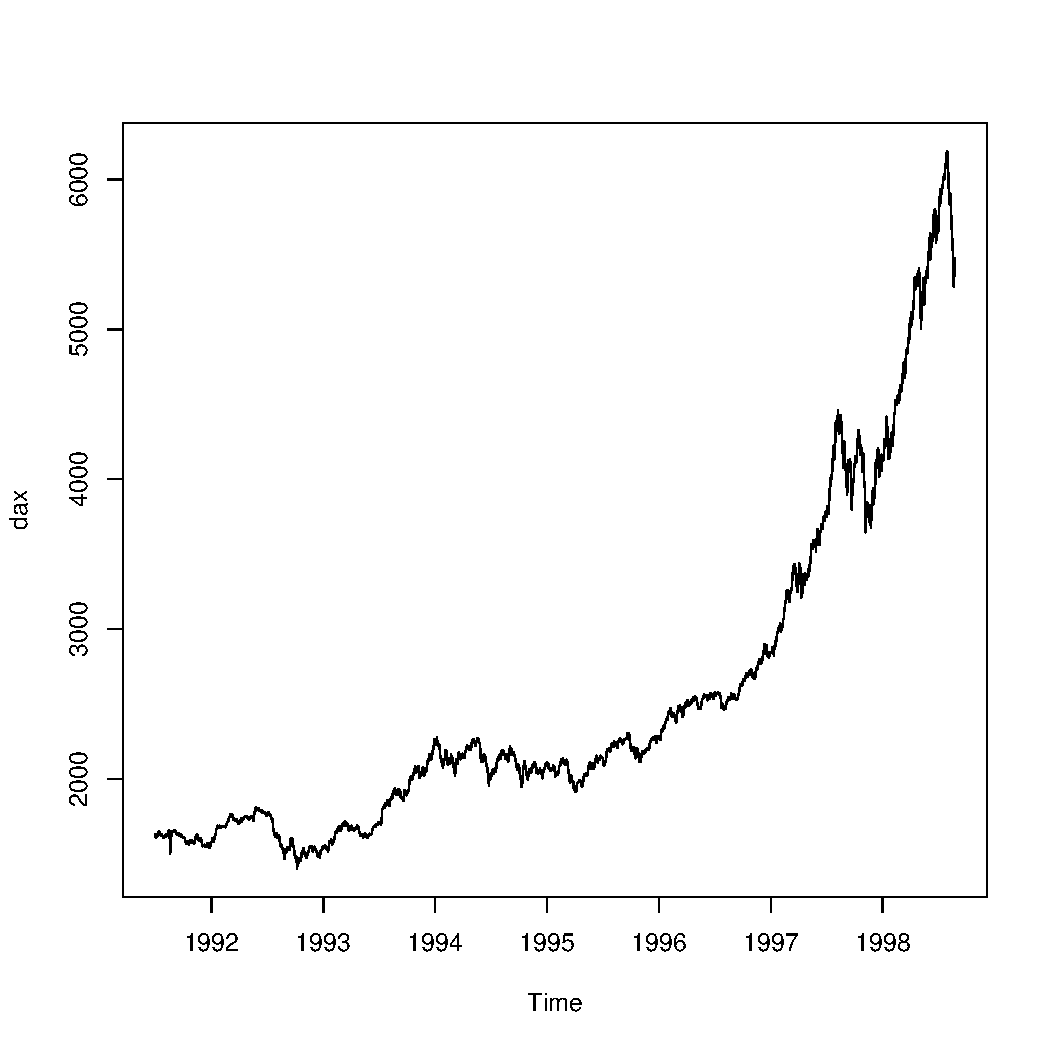
\includegraphics[width=0.95\textwidth]{images/daxPlot.pdf}
%        \end{center}
%      \end{columns}

%\end{frame}

%%%%%%% New frame
%\begin{frame}[allowframebreaks, fragile]
% \frametitle{Customizing the plot}

%To plot more than variables one at a time, use \ttfamily xyplot(): \normalfont
%		\begin{lstlisting}
%# After processing data as in Approach 1
%# load both libraries:
%library(lattice)
%library(zoo)
%data(EuStockMarkets)
%z<-EuStockMarkets
%xyplot(z, screen = c(1,1,1,1), col = 1:4, strip = FALSE)
%legend(1992, 5000, colnames(z), lty = 1, col = 1:4)
%		\end{lstlisting}

%       \begin{center}
%         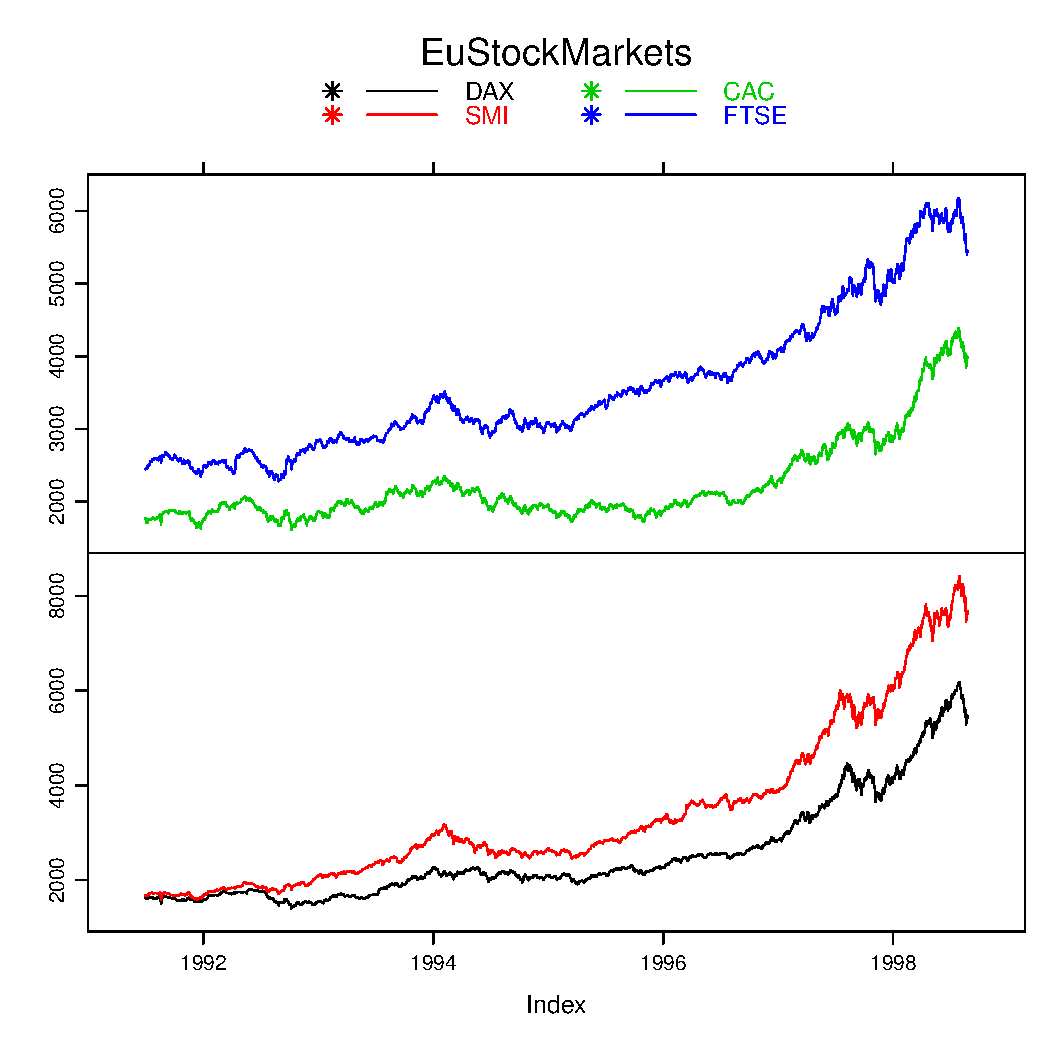
\includegraphics[width=0.85\textwidth]{images/stockPlot2}
%        \end{center}
%\end{frame}

%%%%%%%%%%%%%%%%%%%%%%%%%%%%%%%%%%%%%

\subsection{Multivariate Plots}

%%%%%%%%%%%%%%%%%%%%%%%%%%%%%%%%%%%%%

\begin{frame}[allowframebreaks, fragile]
 \frametitle{Multivariate Time Series Plots}
 \framesubtitle{Approach 1}

To plot more than variables one at a time, use \ttfamily plot(): \normalfont 
	\begin{lstlisting}
# Convert data to a time series via ts() or zoo():
data(airquality)
a<-airquality[, 1:3]
time<-ts(1:nrow(a), start=c(1973, 5), frequency=365)
# If your data is stored as a data frame,
# coerce it to be a matrix via as.matrix()
class(a)
a.mat<-as.matrix(a)


# Make a time series of the two (or more variables)
library(zoo)
name.zoo<-zoo(cbind(a.mat[, 1], a.mat[, 2]))
colnames(name.zoo)<-c("Ozone", "Solar")
#### Plot the variables
plot(name.zoo)
	\end{lstlisting}

       \begin{center}
         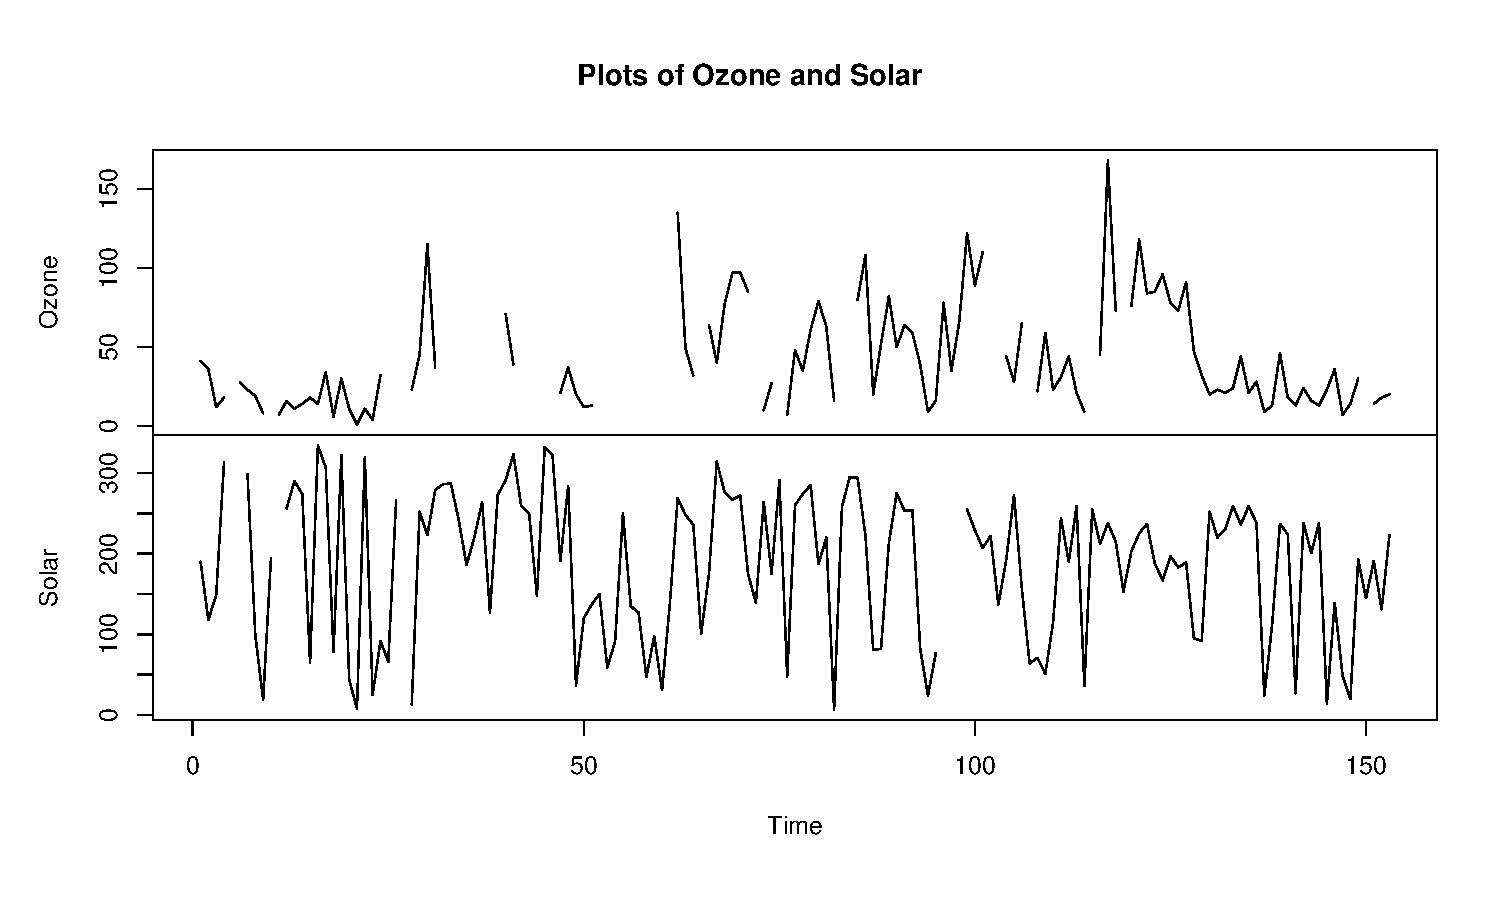
\includegraphics[width=1\textwidth]{images/Mtvsplot1.pdf}
        \end{center}
\end{frame}

%%%%%% New frame
\begin{frame}[fragile]
 \frametitle{Multivariate Time Series Plots}
 \framesubtitle{Approach 2}

To plot more than variables one at a time, use \ttfamily xyplot()\normalfont :
		\begin{lstlisting}
library(lattice)
data(EuStockMarkets)
z<-EuStockMarkets
xyplot(z, screen=c(1,1,2,2), col=1:4, strip=FALSE, key=list(title="EuStockMarkets", 
columns=2, points=FALSE, lines=TRUE, col=1:4, txt=list(colnames(z))))
		\end{lstlisting}
\end{frame}

\begin{frame}[fragile]
 \frametitle{Multivariate Time Series Plots}
 \framesubtitle{Approach 2}

       \begin{center}
         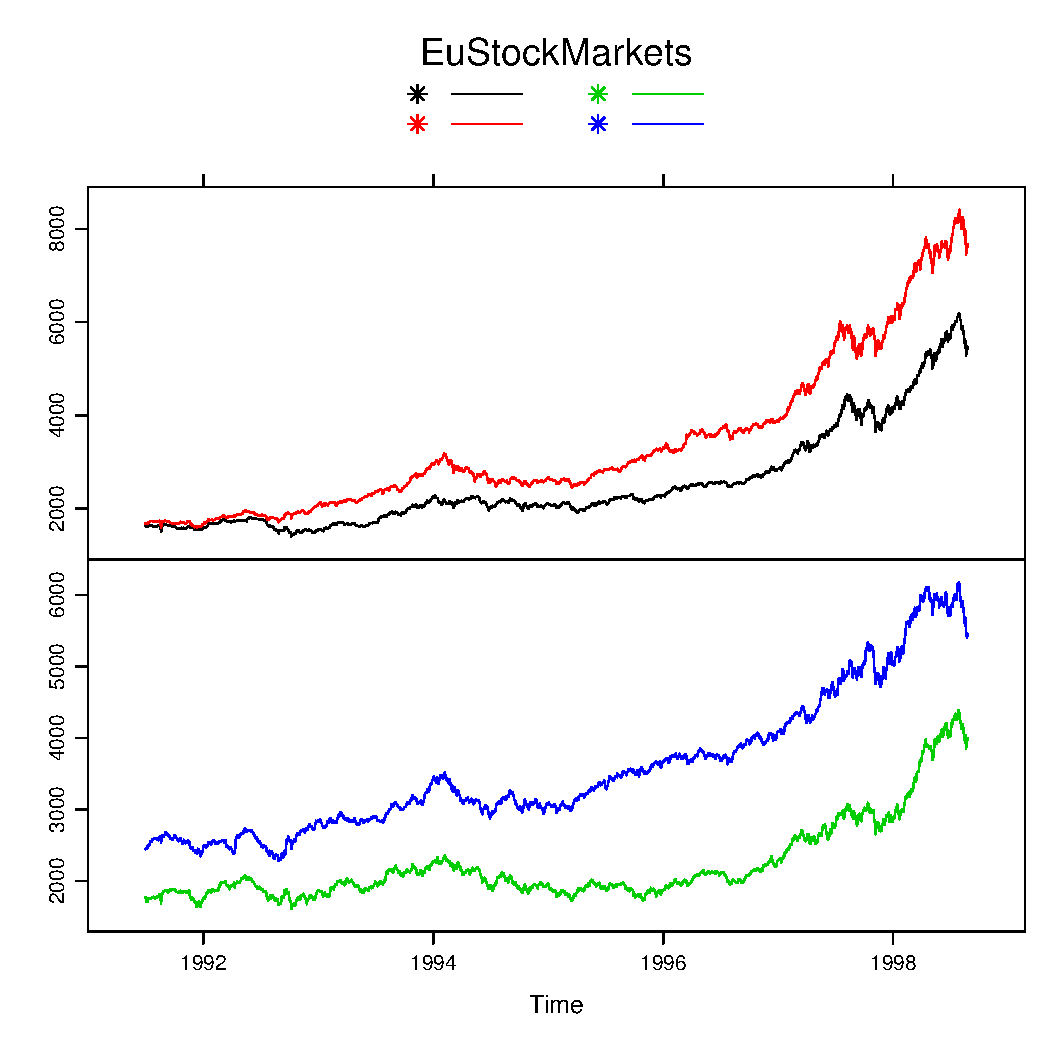
\includegraphics[width=0.58\textwidth]{images/xyplotLattice.pdf}
        \end{center}
\end{frame}



%%%%%% New frame
\begin{frame}[fragile]
 \frametitle{Multivariate Time Series Plots}
 \framesubtitle{Approach 3}

To plot more than variables one at a time, use \ttfamily mvtsplot()\normalfont :\footnote{For documentation, go to: www.jstatsoft.org/v25/c01/paper}
%\begin{itemize}
%	\item For documentation, go to: www.jstatsoft.org/v25/c01/paper 
%	\item Go to: http://www.biostat.jhsph.edu/$\sim$rpeng/RR/mvtsplot/
%	\item Copy the relevant R Code and paste it into the R Console. Press ENTER.
%	\item Plot your data
% \end{itemize}
		\begin{lstlisting}
# Load the R Code for the function
source("http://www.biostat.jhsph.edu/~rpeng/RR/mvtsplot/mvtsplot.R")		
# After processing data as in Approach 1
# Plot the variables
mvtsplot(name.zoo)
# Purple=low, grey=medium, green=high, white=missing values
		\end{lstlisting}
\end{frame}

\begin{frame}[fragile]
 \frametitle{Multivariate Time Series Plots}
 \framesubtitle{Approach 2}

       \begin{center}
         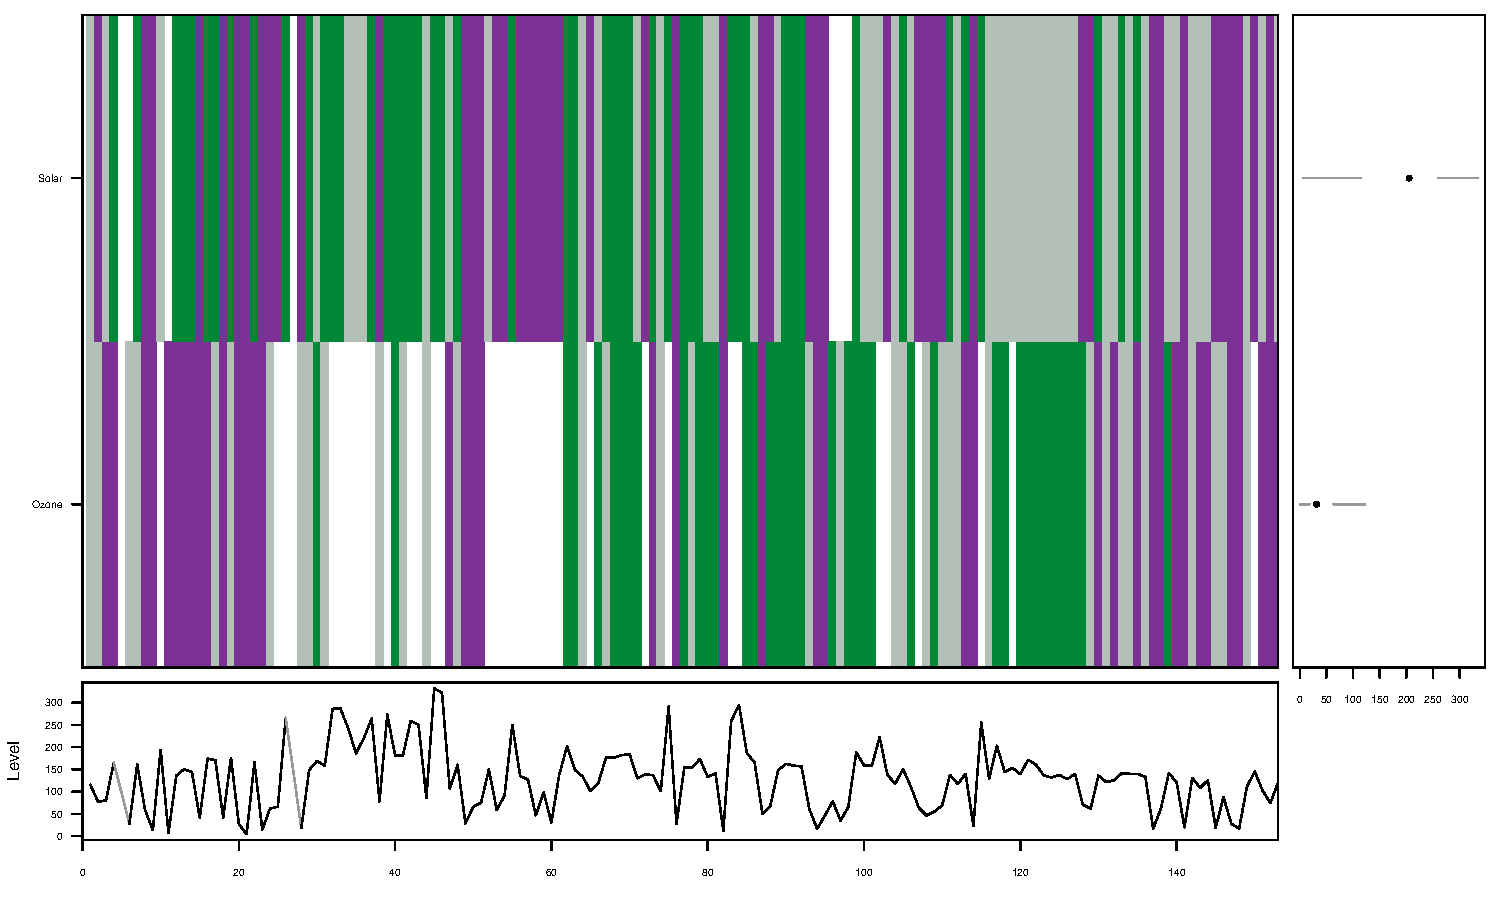
\includegraphics[width=1\textwidth]{images/Mtvsplot2.pdf}
        \end{center}
\end{frame}

%%%%%%% New frame
%\begin{frame}[allowframebreaks, fragile]
% \frametitle{Multivariate Time Series Plots}
% \framesubtitle{Approach 3}
%
%To plot more than variables one at a time, use \ttfamily xyplot(): \normalfont
%		\begin{lstlisting}
%# After processing data as in Approach 1
%# load both libraries:
%library(lattice)
%library(zoo)
%data(EuStockMarkets)
%z<-EuStockMarkets
%xyplot(z, screen = c(1,1,2,2), col = 1:4, strip = FALSE, key = list(title="EuStockMarkets", columns=2, points=FALSE, lines=TRUE, col=1:4, text=list(colnames(z))))
%		\end{lstlisting}
%
%       \begin{center}
%         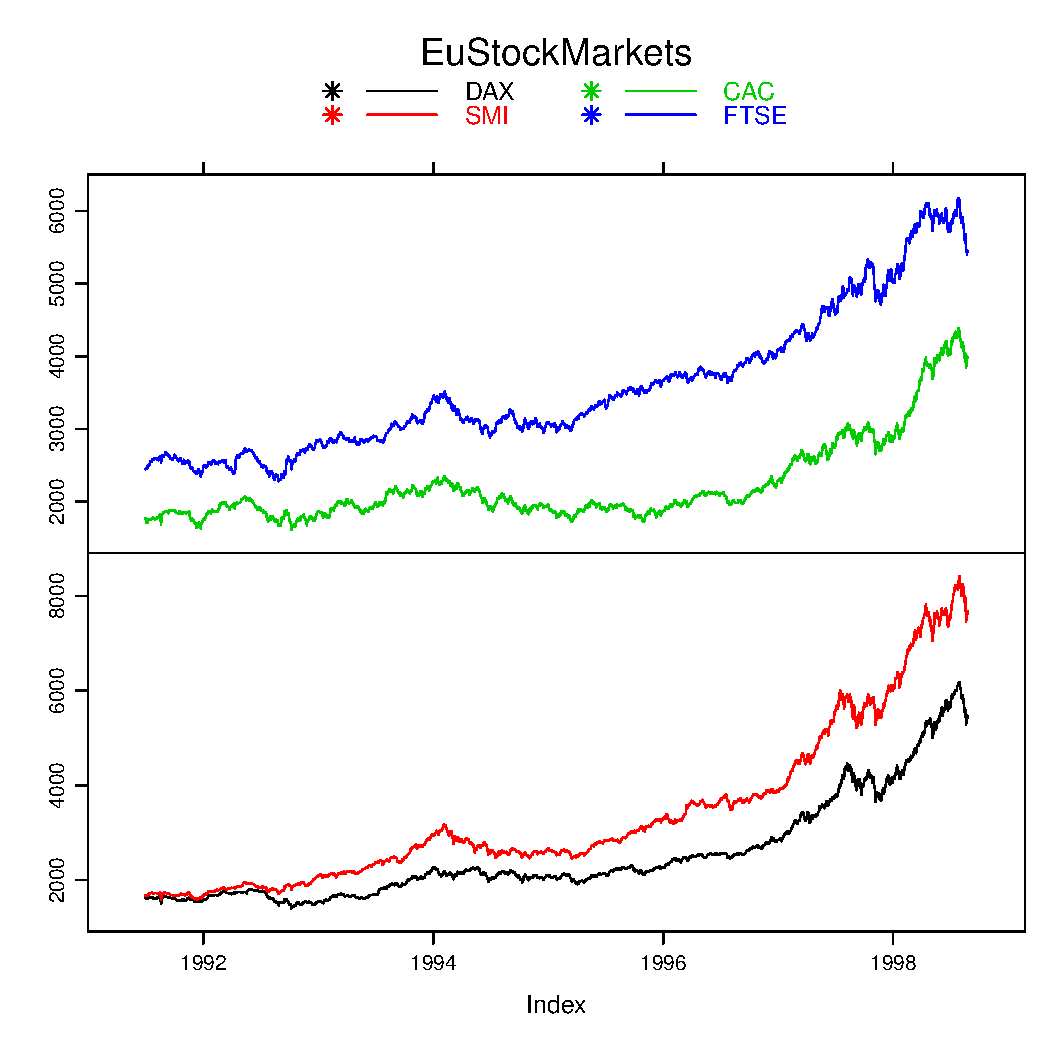
\includegraphics[scale=0.37]{images/stockPlot2.pdf}
%        \end{center}
%\end{frame}
%
%%___________________________________
%\subsection{Customizing Plots}
%%___________________________________

%\begin{frame}[allowframebreaks, fragile]
% \frametitle{Customizing Plots}

%%
%%To plot more than variables one at a time, use \ttfamily xyplot(): \normalfont
%%		\begin{lstlisting}

%%		\end{lstlisting}

%%       \begin{center}
%%         \includegraphics[width=0.85\textwidth]{images/???}
%%        \end{center}
%\end{frame}

% ------------------------------------------------------------
% ------------------------------------------------------------
\subsection{Exercise I}
\begin{frame}
	\frametitle{Exercise I}
	Analyze the \ttfamily EuStockMarkets \normalfont data using the function \ttfamily mtvsplot()\normalfont.  What stands out and why?
\end{frame}